\section{Discrete-Time and Discrete Fourier Transform}
\subsection{Discrete-Time Fourier Transform}
\begin{itemize}
    \item The discrete-time Fourier transform (DTFT) is defined as
    \[
        X(e^{j\omega}) = \sum_{n=-\infty}^{+\infty} x[n] \ e^{-j\omega n}.
    \]
        

    \item Inverse transform
    \begin{align*}
        x[n]
        &= \frac{1}{2\pi} \int_{-\pi}^{+\pi} X(e^{-j\omega}) e^{j\omega n} \mathrm{d}\omega \\
        &= \lim_{\Delta \omega \to 0} \sum_{k} [X(e^{jk\Delta \omega})\frac{\Delta \omega}{2\pi}]e^{jk\Delta \omega n}
    \end{align*}
    Fourier transform decomposes sequences using a linear combination of complex exponentials with incremental amplitudes.

    \item Therefore, the frequency response of a LTI system is the Fourier transform of the impulse response:
    \[
        H(e^{j\omega}) = \sum_{n=-\infty}^{+\infty} h[n] e^{-j\omega n}
    \]
\end{itemize}

\begin{ex}{Frequency Response of the Moving Average System}
The impulse response of the moving average system is
\[
    h[n] = 
    \begin{cases}
        \frac{1}{M_1+M_2+1},    & -M_1 \leq n \leq M_2 \\
        0,  & \text{otherwise}
    \end{cases} 
\]
The frequency response with $M_1=0$ is
\begin{align*}
    H(e^{j\omega}) 
    & = \frac{1}{M_2+1} \sum_{n=0}^{M_2}e^{-j\omega n} \\
    & = \frac{1}{M_2+1} \bigg( \frac{1-e^{-j\omega (M_{2}+1)}}{1-e^{-j\omega}} \bigg) \\
    & = \frac{1}{M_2+1} \frac{(e^{j\omega(M_{2}+1)/2} - e^{-j\omega(M_{2}+1)/2})e^{-j\omega(M_{2}+1)/2}}{(e^{j\omega/2}-e^{-j\omega/2})e^{-j\omega/2}} \\
    & = \frac{1}{M_2+1} \frac{\sin[\omega(M_{2}+1)/2]}{\sin \omega/2}e^{-j\omega M_{2}/2}
\end{align*}
\end{ex}

%% subsection
\subsection{Properties of DTFT}

\paragraph{Periodicity}  If $x[n] \ \xleftrightarrow[]{\mathcal{F}} \ X(e^{j\omega})$, then
\[
    X(e^{j\omega}) =  X(e^{j (\omega+2\pi)}),
\]
\textit{i.e.}, $X(e^{j\omega})$ is $2\pi$-periodic.

\paragraph{Linearity} If $x_1[n] \ \xleftrightarrow[]{\mathcal{F}} \ X_1(e^{j\omega})$ and $x_2[n] \ \xleftrightarrow[]{\mathcal{F}} \ X_2(e^{j\omega})$, then 
\[
    a_1 x_1 [n] + a_2 x_2 [n] \ \xleftrightarrow[]{\mathcal{F}} \ a_1 X_1(e^{j\omega}) + a_2 X_2(e^{j\omega}),
\]
where $a_1$ and $a_2$ are arbitrary real-valued or complex-valued constants.

\paragraph{Translation (Time and Frequency Shifting)} If $x[n] \ \xleftrightarrow[]{\mathcal{F}} \ X(e^{j\omega})$, then the time shifting property is
\[
    x[n - n_{d}] \ \xleftrightarrow[]{\mathcal{F}} \ e^{-j\omega n_{d}} X(e^{j\omega}),
\]
where $n_d$ is an arbitrary integer. Similarly, the frequency shifting property is
\[
    e^{j\omega_d n} x[n]\}  \ \xleftrightarrow[]{\mathcal{F}} \ X(e^{j(\omega-\omega_d)})
\]


\paragraph{Conjugate Symmetry} 
For a real-valued sequence $x[n]$, if $x[n] \ \xleftrightarrow[]{\mathcal{F}} \ X(e^{j\omega})$, then
\[
    X(e^{j\omega}) = X^{*}(e^{-j\omega}), 
\]
where the asterisk * denotes the complex conjugate (not convolution here).

\begin{itemize}
    \item The magnitude of DTFT, $\lvert X(e^{j\omega}) \rvert$ is an \textit{even} function of $\omega$.

    \item The magnitude of DTFT, $\angle X(e^{j\omega})$ is an \textit{odd} function of $\omega$.
\end{itemize}

\begin{dv}{}
Fourier transform:
\[
    X(e^{j\omega}) =  \sum_{n=-\infty}^{+\infty} x[n] e^{-j\omega n}
\]
Replace $\omega$ to $-\omega$:
\[
    X(e^{-j\omega}) =  \sum_{n=-\infty}^{+\infty} x[n] e^{+j\omega n}
\]
Take the complex conjugate of the Fourier transform above: 
\[
    X^{*}(e^{-j\omega}) =  \sum_{n=-\infty}^{+\infty} \underbrace{x^{*}[n]}_{x[n]} e^{-j\omega n}
\]
Since $x[n] \in \mathbb{R}$, the complex conjugate of the Fourier transform is equivalent to Fourier transform:
\[
    X(e^{-j\omega}) = X^{*}(e^{-j\omega})
\]
\rule{\textwidth}{.1ex}
Furthermore, express the Fourier transform in terms of a real part and an imaginary part:
\[
    X(e^{j\omega}) = X_{\mathbb{R}}(e^{j\omega}) + j X_{\mathbb{I}}(e^{j\omega})
\]
The complex conjugate of the Fourier transform is thus
\[
    X^{*}(e^{-j\omega}) = X_{\mathbb{R}}(e^{-j\omega}) - j X_{\mathbb{I}}(e^{-j\omega})
\]
Equate the two expressions above, 
\[
    X_{\mathbb{R}}(e^{j\omega}) = X_{\mathbb{R}}(e^{-j\omega})
\]
\[
    X_{\mathbb{I}}(e^{j\omega}) = -X_{\mathbb{I}}(e^{-j\omega})
\]
That's saying, the real part of the Fourier transform is an \textit{even} function of $\omega$, and the imaginary part of the Fourier transform is an \textit{odd} function of $\omega$.
The magnitude of the Fourier transform is an \textit{even} function of $\omega$; the phase of the Fourier transform is an \textit{odd} function of $\omega$.
\end{dv}

\paragraph{Time Reversal} If $x[n] \ \xleftrightarrow[]{\mathcal{F}} \ X(e^{j\omega})$, then
\[
    x[-n] \ \xleftrightarrow[]{\mathcal{F}} \  X(e^{-j\omega}) = X^*(e^{j \omega}).
\]


\paragraph{Parseval's Theorem}
\[
    \sum_{n=-\infty}^{+\infty} \lvert x[n] \rvert^2 =\frac{1}{2\pi} \int_{-\infty}^{+\infty} \lvert X(e^{j\omega}) \rvert^2 \mathrm{d}\omega 
\]
where $\lvert X(e^{j\omega}) \rvert^2$ is the \textit{energy density spectrum} of the sequence, which determines how the energy is distributed in the frequency domain.

\paragraph{Convolution} If $x_1[n] \ \xleftrightarrow[]{\mathcal{F}} \ X_1(e^{j\omega})$ and $x_2[n] \ \xleftrightarrow[]{\mathcal{F}} \ X_2(e^{j\omega})$, then 
\[
    x_1[n] * x_2[n] \ \xleftrightarrow[]{\mathcal{F}} \ X_1(e^{j\omega}) X_2(e^{j\omega}),
\]
\textit{i.e.}, the convolution of two signals in the time domain is equivalent to the multiplication in the frequency domain. That is saying, for an LTI system, we have 
\[
    y[n] = x[n] * h[n] \ \xleftrightarrow[]{\mathcal{F}} \  Y(e^{j\omega}) = X(e^{j\omega})H(e^{j\omega}).
\]
    

%% subsection
\subsection{Common DTFT Pairs}
\begin{table}[H]
    \centering
    \begin{tabular}{c c}
    \toprule
    $x[n]$    & $X(e^{j\omega})$ \\ 
    \midrule
        $\delta[n]$     &   1  \\[.5em]
        
        1   &   $2\pi \sum_{n=-\infty}^{+\infty} \delta(\omega-2\pi n)$ \\[.5em]
        
        $u[n]$  &   $\frac{e^{j\omega}}{e^{j\omega}-1} \sum_{n=-\infty}^{+\infty} \pi \delta(\omega-2\pi n)$ \\[.5em]
        
        $a^n u[n]$, $\lvert a \rvert <1$    &   $\frac{e^{j\omega}}{e^{j\omega}-a}$ \\[.5em]

        $-a^n u[-n-1]$, $\lvert a \rvert >1$    &   $\frac{e^{j\omega}}{e^{j\omega}-a}$ \\[.5em]

        $a^{\lvert n \rvert}$, $\lvert a \rvert <1$     &   $\frac{1-a^2}{1-2a\cos\omega+a^2}$ \\[.5em]

        $\cos(\omega_0 n)$    &   $\pi \sum_{k=\infty}^{+\infty} [\delta(\omega -\omega_0 - 2\pi k) + \delta(\omega +\omega_0 - 2\pi k)]$ \\[.5em]

        $\sin(\omega_0 n)$    &   $j\pi \sum_{k=\infty}^{+\infty} [\delta(\omega + \omega_0 - 2\pi k) - \delta(\omega - \omega_0 - 2\pi k)]$ \\[.5em]

        $u[n] - u[n-M]$ &   $e^{-j\omega(M-1)/2} (\frac{\sin(M\omega/2)}{\sin(\omega/2)})$\\[.5em]
    \bottomrule
    \end{tabular}
\end{table}

%% subsection
\subsection{From DTFT to Discrete Fourier Transform (DFT)}

\paragraph{Sampling the frequency domain in DTFT leads to the DFT}
\begin{itemize}
    \item The discrete-time Fourier transform (DTFT) requires a continuity of its frequency $\omega$.

    \item If we sample the frequency $\displaystyle \omega = \frac{2\pi k}{N}$ where $k \in [0, N-1]$ from DTFT, the sampled signal $X[k]$ is
    \[
        X[k] = X(e^{j\omega})\lvert_{\omega = \frac{2\pi k}{N}} \ = \ \sum_{n=0}^{N-1} x[n] \ e^{-j {\color{red}\frac{2\pi k}{N}} n}.
    \]
    This process is the \textbf{discrete Fourier transform} (DFT). DFT is a sequence with the same duration as the discrete-time sequence, with a sampled frequency axis.

    \item The \textbf{inverse discrete Fourier transform} is
    \[
        x[n] = \frac{1}{N} \sum_{k=0}^{N-1} X[k] \ e^{{j \color{red}\frac{2\pi k}{N}} n}.
    \]
    DFT is sufficient to reconstruct the original discrete-time series, given the discrete-time series is of finite duration.
\end{itemize}

\paragraph{What happens when we sample the frequency domain?} Let $\widetilde{X}(e^{j\omega})$ denote the signal results from sampling $X(e^{j\omega})$ at the frequency $\displaystyle \omega = \frac{2\pi k}{N}$ (where $k \in [0, N-1]$):
\[
    \widetilde{X}(e^{j\omega}) = X(e^{j\omega})  \ \overbrace{\sum_{k=-\infty}^{+\infty} \delta \left(\omega-\frac{2\pi k}{N} \right)}^{\text{\color{gray} sampler}},
\]
by applying the inverse Fourier transform of $\widetilde{X}(e^{j\omega})$,
\[
    \widetilde{x}[n] = N \sum_{k=-\infty}^{+\infty} x[n-kN],
\]
for which we now obtained a periodic signal (in its time domain). This tells us that \textbf{sampling the Fourier transform in the \textit{frequency} domain corresponds to the periodization in the \textit{time} domain}.

\begin{figure}[H]
\centering
\begin{subfigure}{\textwidth}
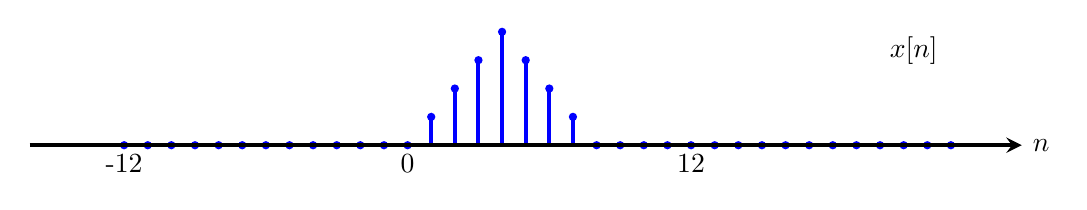
\begin{tikzpicture}[scale = 0.6]
    % Parameters
    \def\N{12} % Period of the signal
    \def\signalLength{8} % Length of the non-zero signal within each period

    % Draw the periodic signal
    \foreach \k in {-1, 0, 1} { % Loop over different periods
        \foreach \n in {0, 1, ..., 11} { % Loop over the entire period
            % Define the height with x = 4 being the highest
            \ifnum\k=0
            \ifnum\n<9
                \pgfmathsetmacro{\height}{0.6*(4 - abs(\n - 4))} % Set non-zero heights for n=0 to n=8
            \else
            \pgfmathsetmacro{\height}{0} % Set height to 0 for n=9 to n=11
            \fi
            \else
                \pgfmathsetmacro{\height}{0} % Set height to 0 for n=9 to n=11
            \fi
            
            \draw[thick, line width=0.5mm, blue] (0.5*\k*\N + 0.5*\n, 0) -- (0.5*\k*\N + 0.5*\n, \height); % Draw vertical line
            \fill[blue] (0.5*\k*\N + 0.5*\n, \height) circle (2.5pt); % Mark the top of the bar
        }
    }
    % Draw the horizontal axis
    \draw[-stealth, line width=.5mm] (-8, 0) -- (13, 0) node[right] {$n$};
    % Add key points and labels
    \foreach \x in {-12, 0, 12} {
        \node[below] at (0.5*\x, 0) {\x};
    }

    \node[right] at (10, 2) {$\displaystyle \boldsymbol{x[n]}$};
\end{tikzpicture}
\caption{Finite sequence of $x[n]$}
\end{subfigure}

\begin{subfigure}{\textwidth}
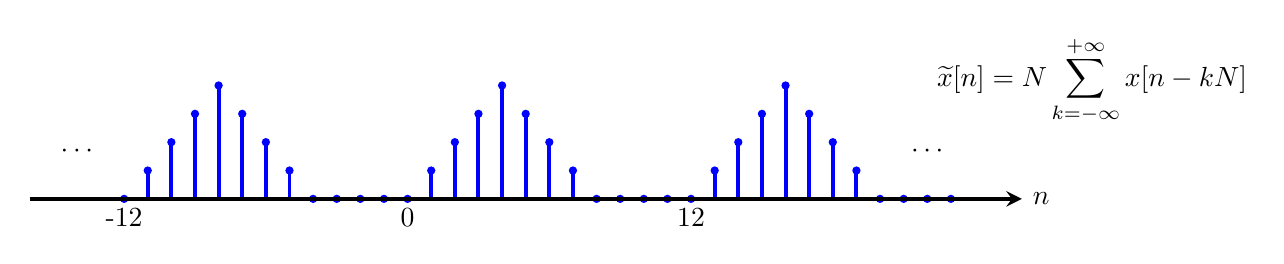
\begin{tikzpicture}[scale=0.6]
    % Parameters
    \def\N{12} % Period of the signal
    \def\signalLength{8} % Length of the non-zero signal within each period

    % Draw the periodic signal
    \foreach \k in {-1, 0, 1} { % Loop over different periods
        \foreach \n in {0, 1, ..., 11} { % Loop over the entire period
            % Define the height with x = 4 being the highest
            \ifnum\n<9
                \pgfmathsetmacro{\height}{0.6*(4 - abs(\n - 4))} % Set non-zero heights for n=0 to n=8
            \else
                \pgfmathsetmacro{\height}{0} % Set height to 0 for n=9 to n=11
            \fi
            
            \draw[thick, line width=0.5mm, blue] (0.5*\k*\N + 0.5*\n, 0) -- (0.5*\k*\N + 0.5*\n, \height); % Draw vertical line
            \fill[blue] (0.5*\k*\N + 0.5*\n, \height) circle (2.5pt); % Mark the top of the bar
        }
    }

    % Draw the horizontal axis
    \draw[-stealth, line width=.5mm] (-8, 0) -- (13, 0) node[right] {$n$};

    % Add key points and labels
    \foreach \x in {-12, 0, 12} {
        \node[below] at (0.5*\x, 0) {\x};
    }
    \node[right] at (11, 2.5) {$\displaystyle \boldsymbol{\widetilde{x}[n] = N \sum_{k=-\infty}^{+\infty} x[n-kN]}$};

    \node at (11, 1) {$\cdots$};
    \node at (-7, 1) {$\cdots$};
\end{tikzpicture}
\caption{Periodic sequence $\widetilde{x}[n]$ corresponding to the sampling of Fourier transform of $x[n]$}
\end{subfigure}
\caption{Illustration of a discrete-time signal $x[n]$ and its periodic extension $\widetilde{x}[n]$.}
\end{figure}

%% subsection
\subsubsection{Power Spectral Density of DFT}
Power spectral density (PSD, also known as the power spectrum) quantifies the power of the signal per unit frequency.
\[
    PSD[k] = \frac{1}{N}\lvert X[k] \rvert^2 = \frac{1}{N} \bigg \lvert  \sum_{n=0}^{N-1} x[n] e^{-j 2 \pi kn/N}\bigg \rvert^2. 
\]

\subsubsection{Zero-Padding}
Zero padding is the process of appending extra zeros to the end of a signal before performing DFT. Mathematically,
\[
    \hat{x}[n] = 
    \begin{cases}
        x[n], & \text{for} \ n = 0, ..., N-1\\
        0, & \text{for} \ n = N, ..., M
    \end{cases},
\]
where $M$, $N$ are two integers, and $M>N$. \\

Zero padding causes DTF to be evaluated from DTFT with more samples in $\omega_k$, \textit{i.e.}, denser frequency samples are obtained, hence, a smoother frequency spectrum.

\begin{figure}[H]
    \centering
    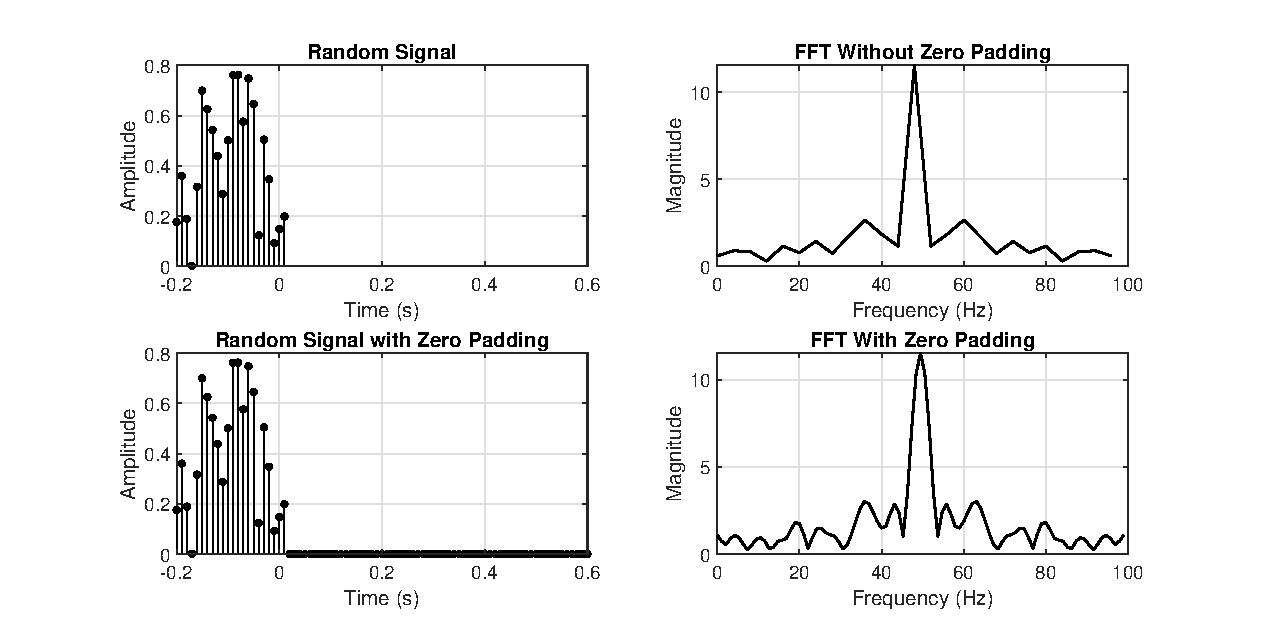
\includegraphics[width=\linewidth]{Digital Biosignal Processing/images/zero_padding.eps}
    \caption{Effect of zero-padding on the resolution of the Fourier Transform of a random signal.}
    \label{fig:zero-padding}
\end{figure}

%% subsection
\subsection{Summary}
\begin{figure}[H]
    \centering
    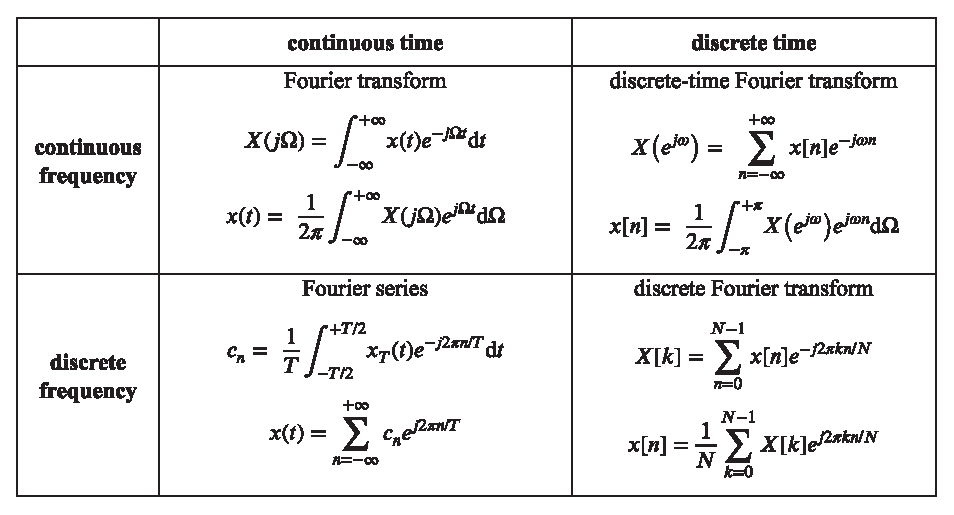
\includegraphics{images/summary_of_FTs.eps}
\end{figure}

\subsection{Example Questions}
%==============================================%
\begin{q}{}
Consider the discrete-time signal $x[n] = e^{\frac{j\pi n}{2}}$ and a linear, time-invariant system with transfer function $H(e^{-j\omega}) = e^{-j \omega}$. The output $y[n]$ of this system when the input $x[n]$ is:

\begin{enumerate}[label=(\alph*)]
    \item $y[n] = 0$
    \item $y[n] = -je^{\frac{j\pi n}{2}}$
    \item $y[n] = je^{\frac{j\pi n}{2}}$
    \item $y[n] = x[n] \cdot \lvert H(e^{\frac{j \pi}{2}})\rvert$
    \item $y[n] = x[n]$
\end{enumerate}
\begin{flushright}
\begin{blueenv}
    ANS: (b)
\end{blueenv}
\end{flushright}
\end{q}
%==============================================%
\begin{q}{}
Consider the deterministic discrete-time signal $x[n] = \delta[n] - \delta[n-1]$ which has a length of $N = 2$ samples. Which of the following expressions for the Discrete Fourier Transform (DFT) $X[k]$ (for $k = 0, 1$) of $x[n]$ is correct?

\begin{enumerate}[label=(\alph*)]
    \item $X[0] = 0, \, X[1] = 2$
    \item $X[0] = 1, \, X[1] = -1$
    \item $X[0] = j, \, X[1] = -j$
    \item $X[0] = e^{j\frac{\pi}{3}}, \, X[1] = e^{j\frac{\pi}{4}}$
    \item $X[0] = 1, \, X[1] = -j$
\end{enumerate}
\begin{flushright}
\begin{blueenv}
    ANS: (a)
\end{blueenv}
\end{flushright}
\end{q}
%==============================================%
\begin{q}{}
    Given the following discrete-time signal:
    \[
        x[n] = 
        \begin{cases}
            1, & n=0 \\
            -3, & n=1 \\
            -1, & n=2 \\
            0, & n=3
        \end{cases}
    \]
    \begin{enumerate}[label=(\alph*)]
        \item Compute the discrete-time Fourier transform $X(e^{j\omega})$.
        \begin{flushright}
        \begin{blueenv}
            ANS: $X(e^{j\omega}) = 1 - 3e^{-j\omega} - e^{-j2\omega}$.
        \end{blueenv}
        \end{flushright}
        
        \item Compute the discrete Fourier transform $X[k]$ over four points.
        \begin{flushright}
        \begin{blueenv}
            ANS: $X[k] = 
            \begin{cases}
                -3, & k = 0\\
                2+3j, & k = 1\\
                3, & k=2 \\
                2-3j, & k=3
            \end{cases}.$
        \end{blueenv}
        \end{flushright}
        
    \end{enumerate}
    % {\color{blue}
    %     \paragraph{Answer (a)}
    %     \begin{align*}
    %         X(e^{j\omega}) 
    %         & = \sum_{n=0}^{4} x[n] e^{-j\omega n} \\
    %         & = 1 - 3e^{-j\omega} - e^{-j2\omega}
    %     \end{align*}
    % }
    % {\color{blue}
    %     \paragraph{Answer (b)}
    %     \begin{align*}
    %         X[k] 
    %         & = X(e^{j\omega})\lvert_{\omega = \frac{2\pi k}{4}} \\
    %         & = \begin{cases}
    %             -3, & k = 0\\
    %             2+3j, & k = 1\\
    %             3, & k=2 \\
    %             2-3j, & k=3
    %         \end{cases}.
    %     \end{align*}
    % }
\end{q}





